\chapter{Significance plots}
\label{sec:appsignificance}

\section{Direct slepton production}

\subsection{Low level features}

\newpage

\begin{figure}[H]
    \centering
    \begin{subfigure}[t!]{0.49\textwidth}
    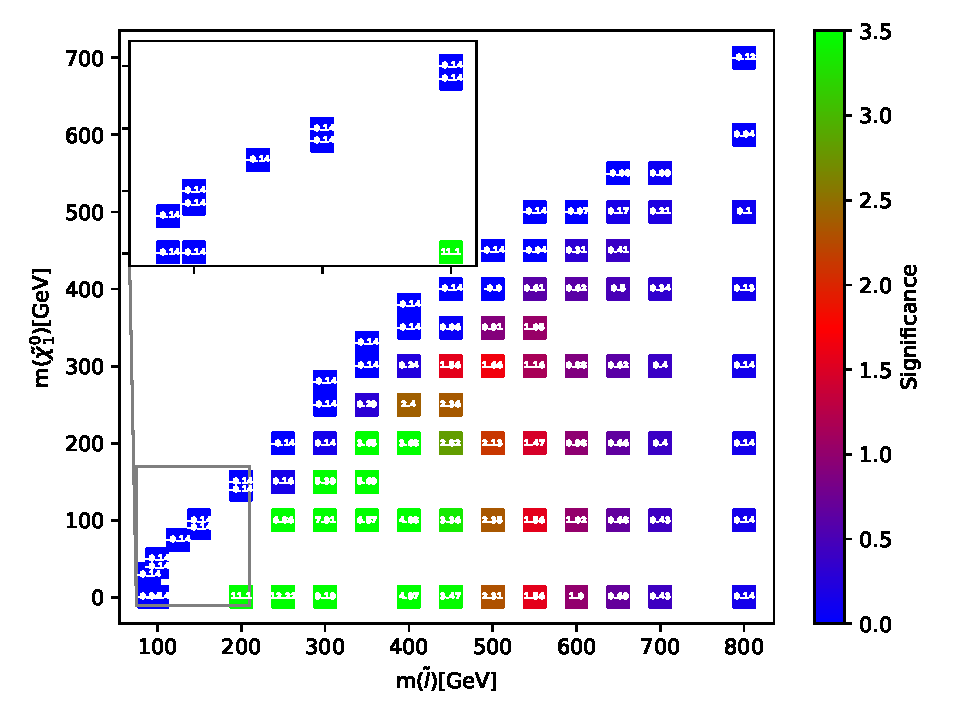
\includegraphics[width = \textwidth]{Figures/Significances/significanceCutandCount_slepslep_all.pdf}
    \caption{Cut and count.}
        \label{fig:signLowSlepSlepcandc}
    \end{subfigure}
    \\
    \begin{subfigure}[t!]{0.49\textwidth}
    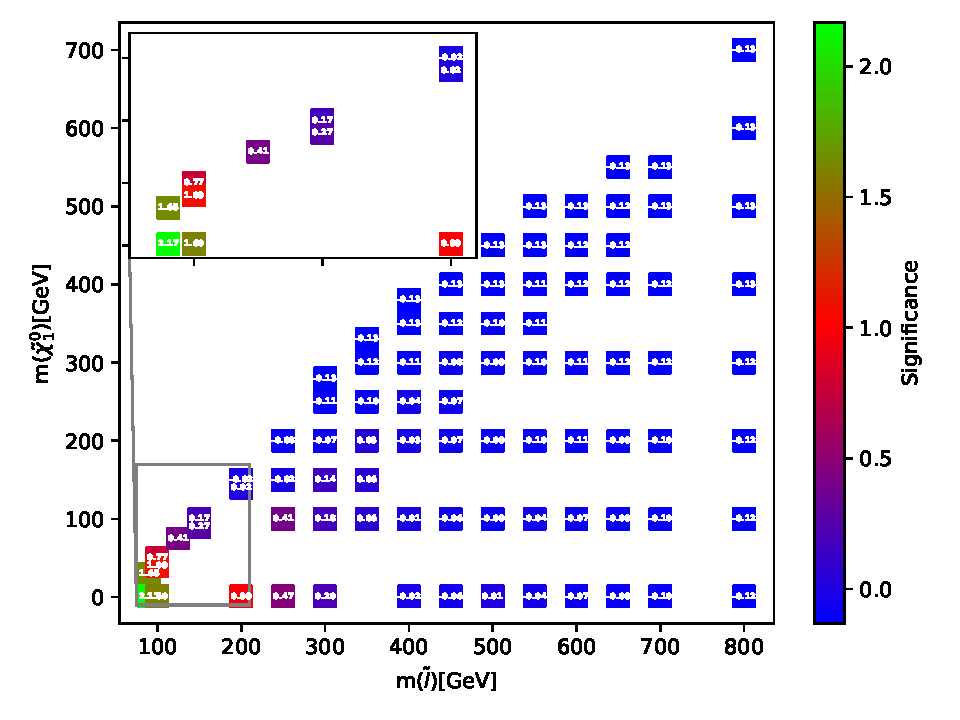
\includegraphics[width = \textwidth]{Figures/Significances/significance_BDT_slepslep_Low_level.pdf}
    \caption{Boosted Decision Tree.}
        \label{fig:signLowSlepSlepBDT}
    \end{subfigure}      
    \begin{subfigure}[t!]{0.49\textwidth}
    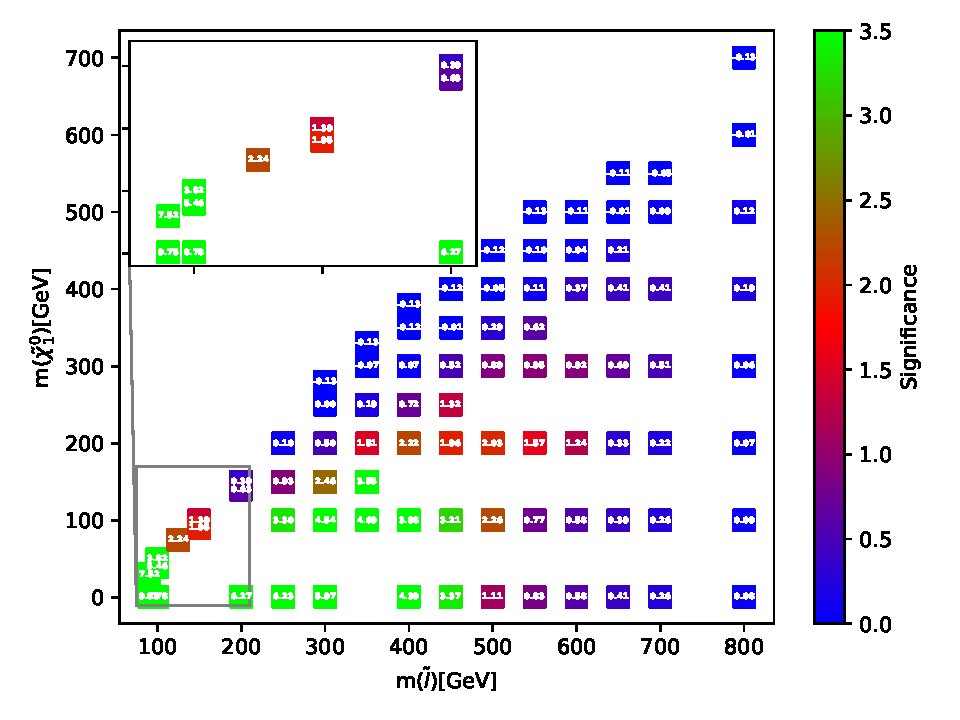
\includegraphics[width = \textwidth]{Figures/Significances/significance_NN_slepslep_Low_level.pdf}
    \caption{Neural Network.}
        \label{fig:signLowSlepSlepNN}
    \end{subfigure}
    \caption{Significance plots for direct slepton production where low level features are used during training the ML models.}
    \label{fig:signLowSlepSlep}
\end{figure}


\subsection{High level features}

\begin{figure}[H]
    \centering
    \begin{subfigure}[t!]{0.49\textwidth}
    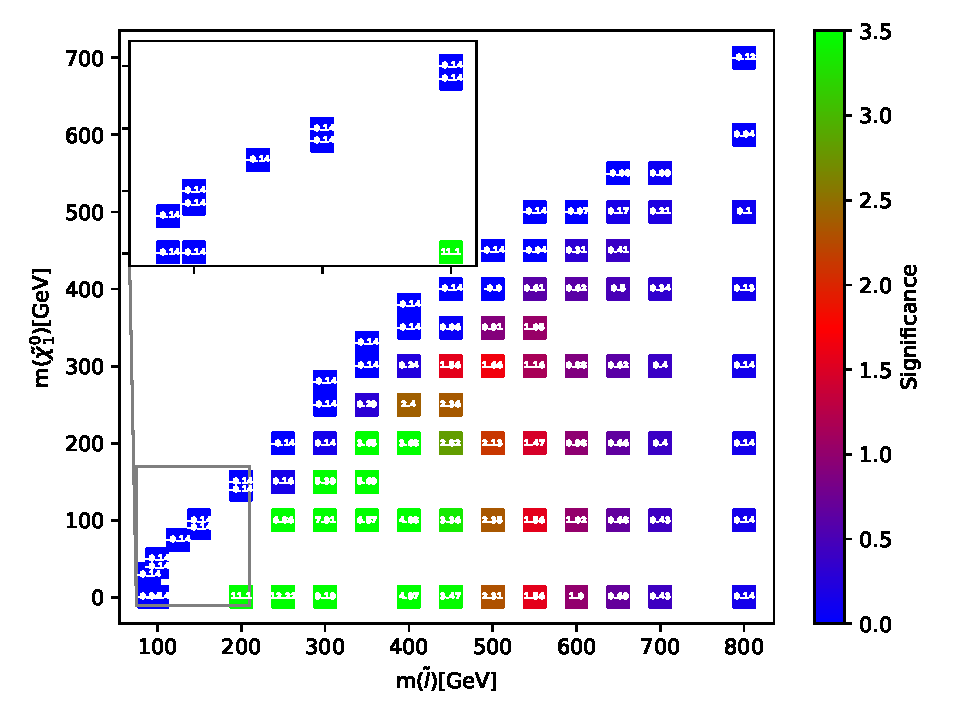
\includegraphics[width = \textwidth]{Figures/Significances/significanceCutandCount_slepslep_all.pdf}
    \caption{Cut and count.}
        \label{fig:signHighSlepSlepcandc}
    \end{subfigure}
    \\
    \begin{subfigure}[t!]{0.49\textwidth}
    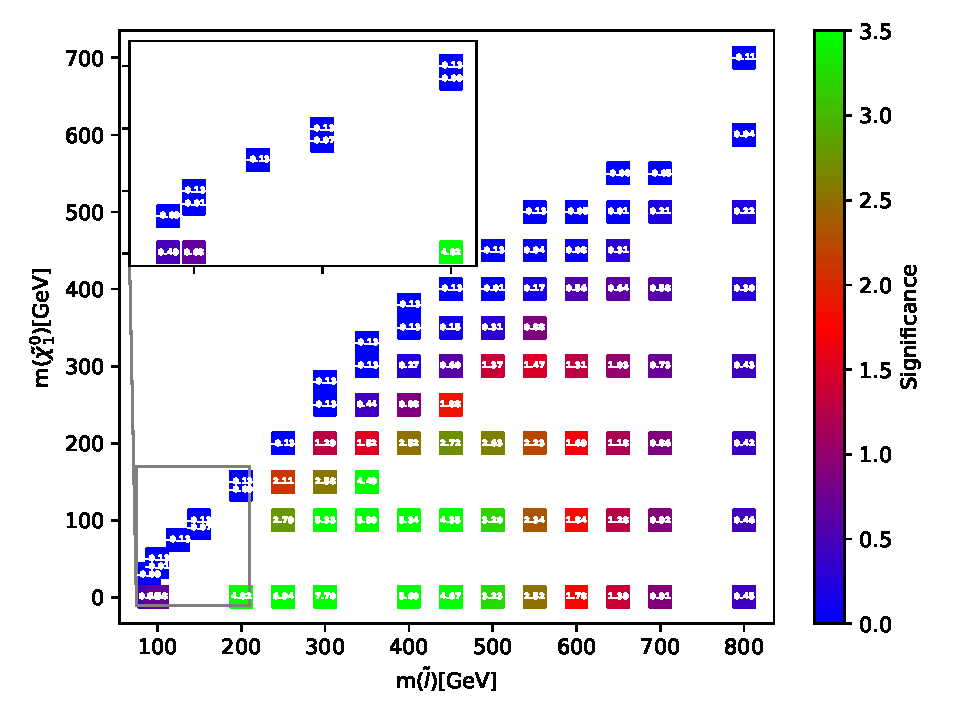
\includegraphics[width = \textwidth]{Figures/Significances/significance_BDT_slepslep_High_level.pdf}
    \caption{Boosted Decision Tree.}
        \label{fig:signHighSlepSlepBDT}
    \end{subfigure}      
    \begin{subfigure}[t!]{0.49\textwidth}
    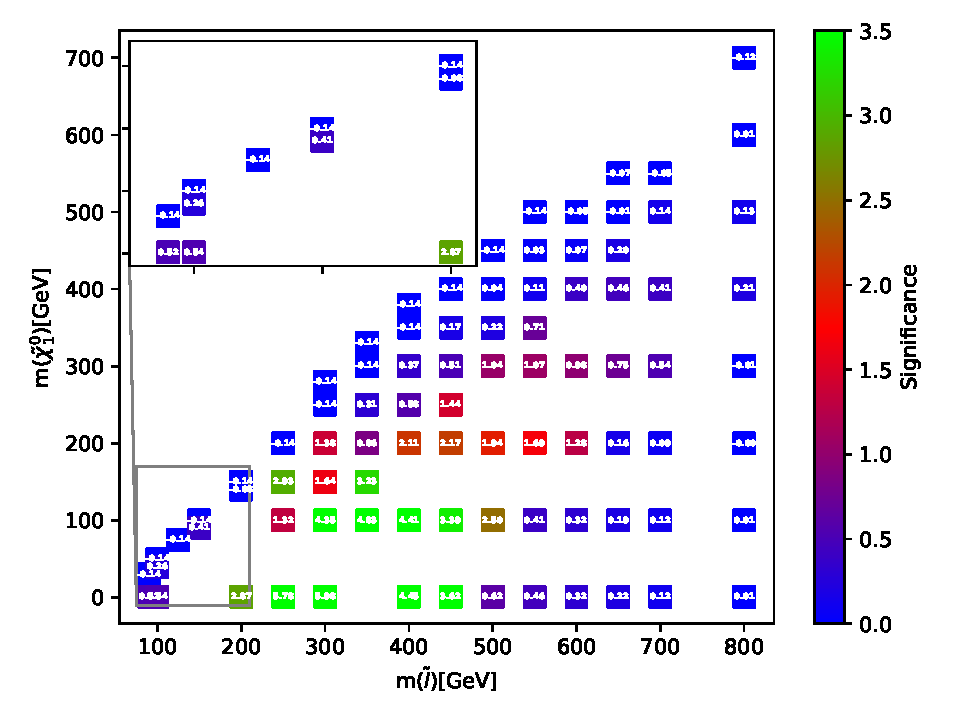
\includegraphics[width = \textwidth]{Figures/Significances/significance_NN_slepslep_High_level.pdf}
    \caption{Neural Network.}
        \label{fig:signHighSlepSlepNN}
    \end{subfigure}
    \caption{Significance plots for direct slepton production where high level features are used during training the ML models.}
    \label{fig:signHighSlepSlep}
\end{figure}















\section{Chargino pair via slepton or sneutrino}

\subsection{Low level features}

\begin{figure}[H]
    \centering
    \begin{subfigure}[t!]{0.49\textwidth}
    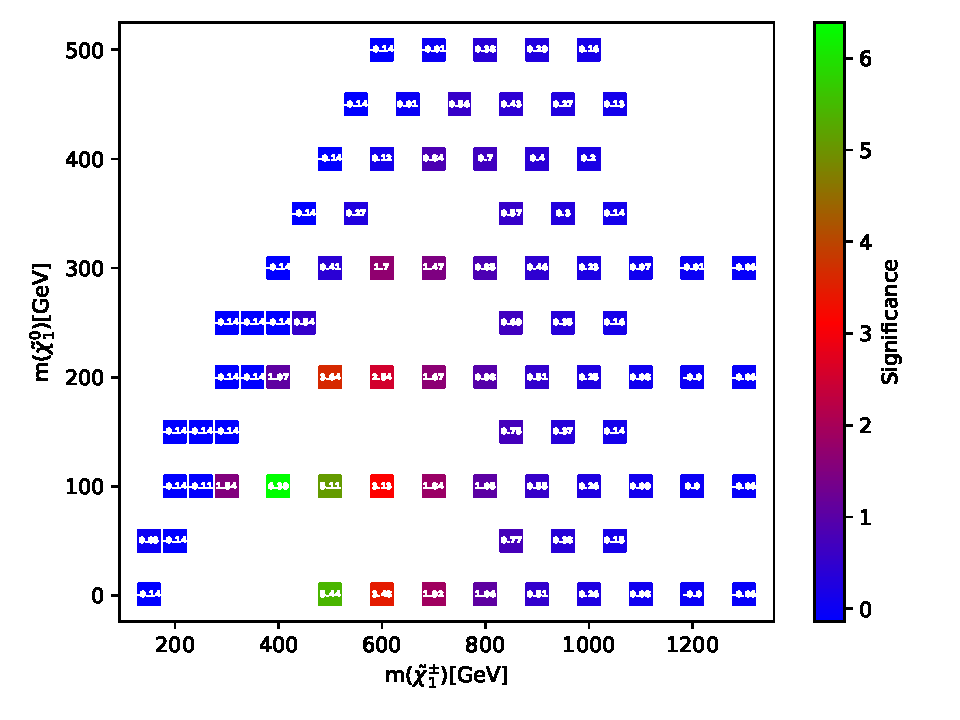
\includegraphics[width = \textwidth]{Figures/Significances/significanceCutandCount_slepsnu_all.pdf}
    \caption{Cut and count.}
        \label{fig:signLowslepsnucandc}
    \end{subfigure}
    \\
    \begin{subfigure}[t!]{0.49\textwidth}
    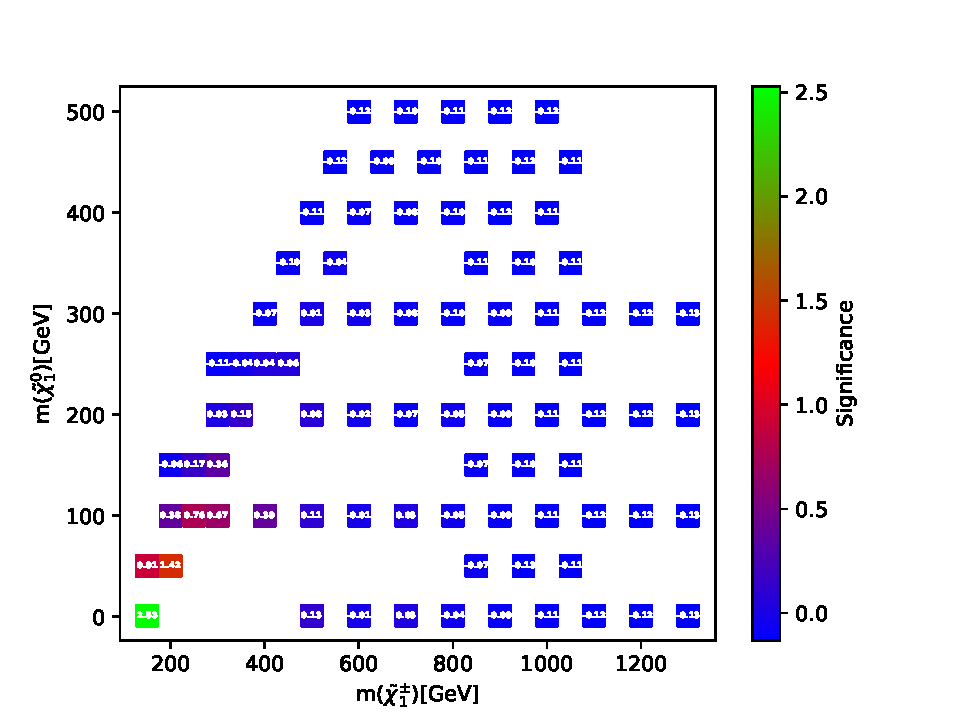
\includegraphics[width = \textwidth]{Figures/Significances/significance_BDT_slepsnu_Low_level.pdf}
    \caption{Boosted Decision Tree.}
        \label{fig:signLowslepsnuBDT}
    \end{subfigure}      
    \begin{subfigure}[t!]{0.49\textwidth}
    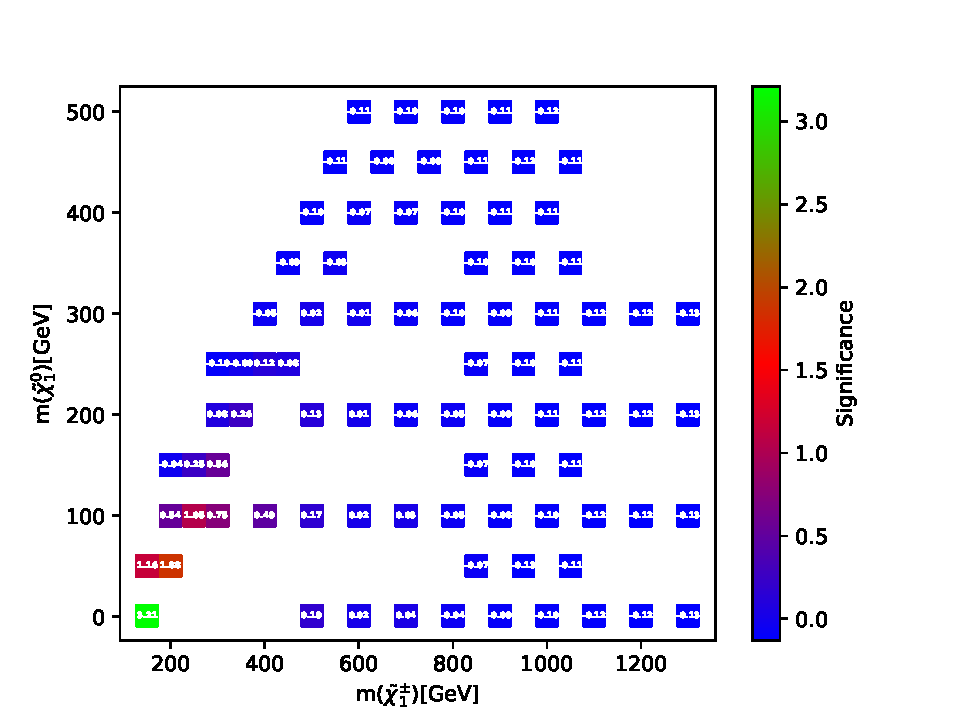
\includegraphics[width = \textwidth]{Figures/Significances/significance_NN_slepsnu_Low_level.pdf}
    \caption{Neural Network.}
        \label{fig:signLowslepsnuNN}
    \end{subfigure}
    \caption{Significance plots for chargino production with slepton/sneutrino-mediated-decay where low level features are used during training the ML models.}
    \label{fig:signLowslepsnu}
\end{figure}


\subsection{High level features}

\begin{figure}[H]
    \centering
    \begin{subfigure}[t!]{0.49\textwidth}
    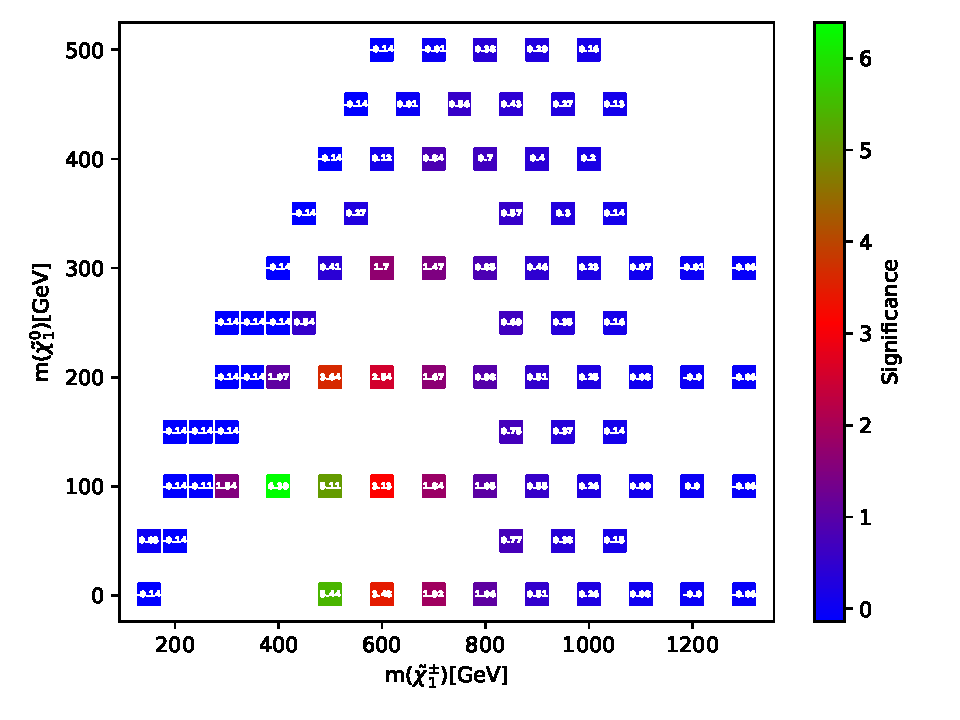
\includegraphics[width = \textwidth]{Figures/Significances/significanceCutandCount_slepsnu_all.pdf}
    \caption{Cut and count.}
        \label{fig:signHighslepsnucandc}
    \end{subfigure}
    \\
    \begin{subfigure}[t!]{0.49\textwidth}
    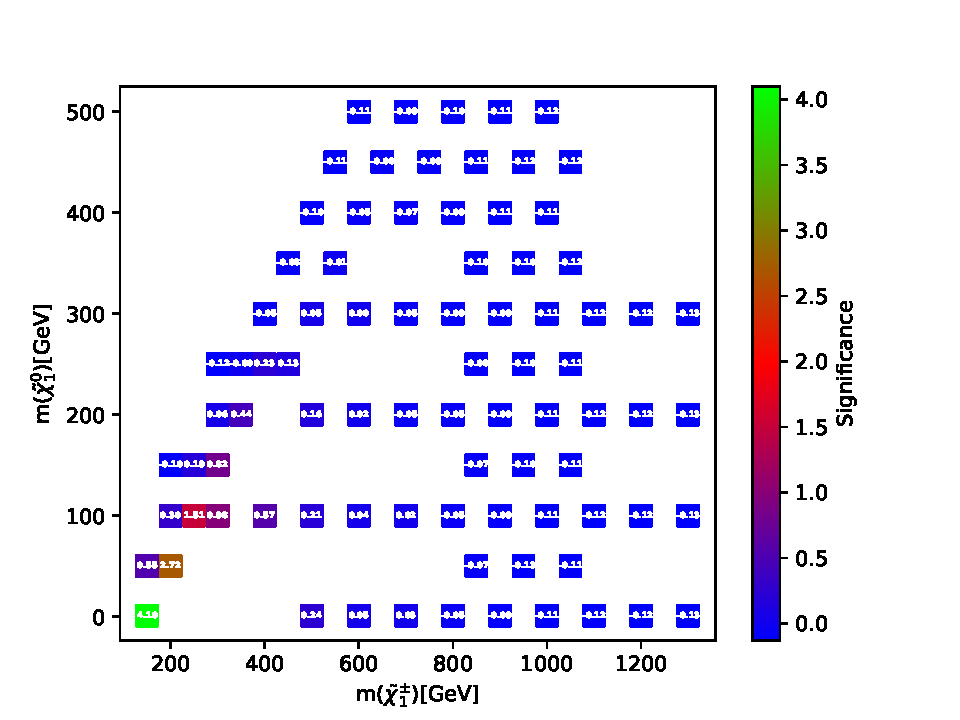
\includegraphics[width = \textwidth]{Figures/Significances/significance_BDT_slepsnu_High_level.pdf}
    \caption{Boosted Decision Tree.}
        \label{fig:signHighslepsnuBDT}
    \end{subfigure}      
    \begin{subfigure}[t!]{0.49\textwidth}
    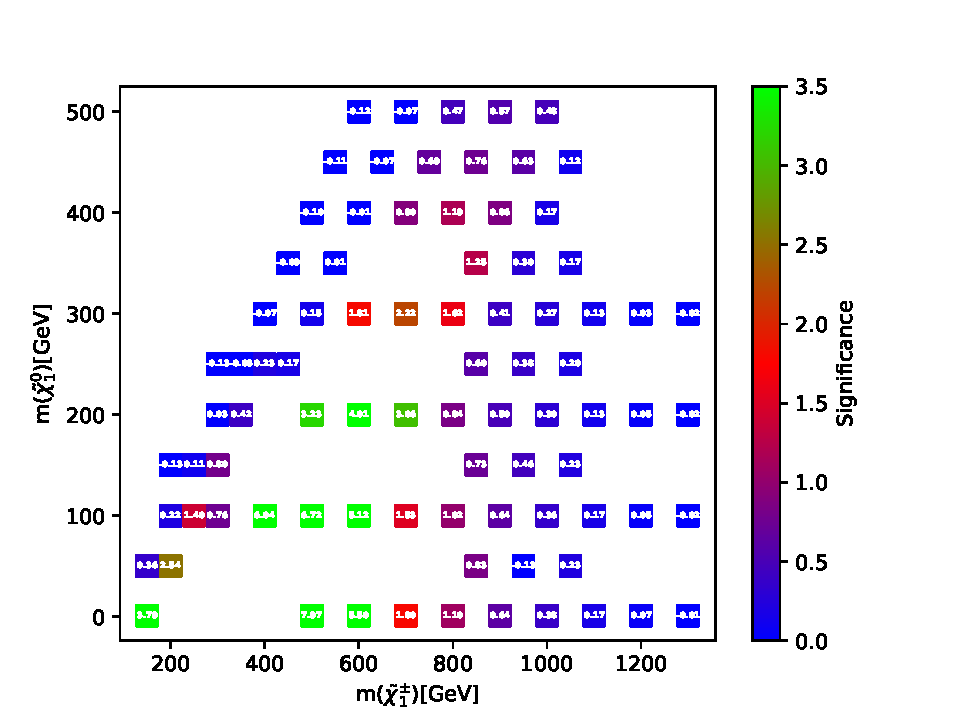
\includegraphics[width = \textwidth]{Figures/Significances/significance_NN_slepsnu_High_level.pdf}
    \caption{Neural Network.}
        \label{fig:signHighslepsnuNN}
    \end{subfigure}
    \caption{Significance plots for chargino production with slepton/sneutrino-mediated-decay where high level features are used during training the ML models.}
    \label{fig:signHighslepsnu}
\end{figure}







\section{Chargino pair via W-bosons}

\subsection{Low level features}

\begin{figure}[H]
    \centering
    \begin{subfigure}[t!]{0.49\textwidth}
    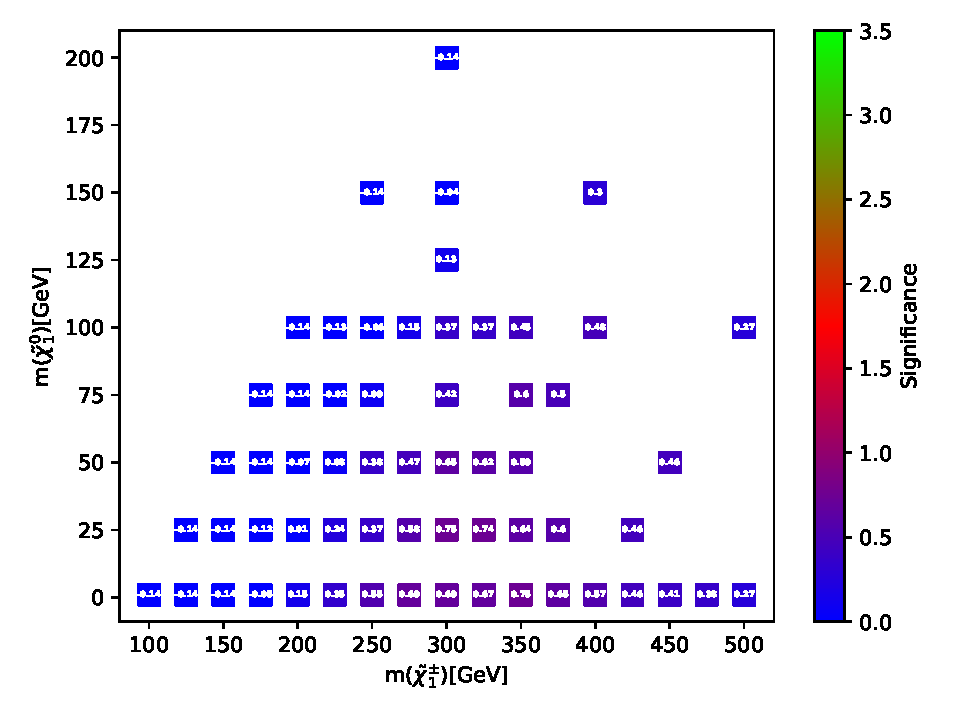
\includegraphics[width = \textwidth]{Figures/Significances/significanceCutandCount_WW_all.pdf}
    \caption{Cut and count.}
        \label{fig:signLowWWcandc}
    \end{subfigure}
    \\
    \begin{subfigure}[t!]{0.49\textwidth}
    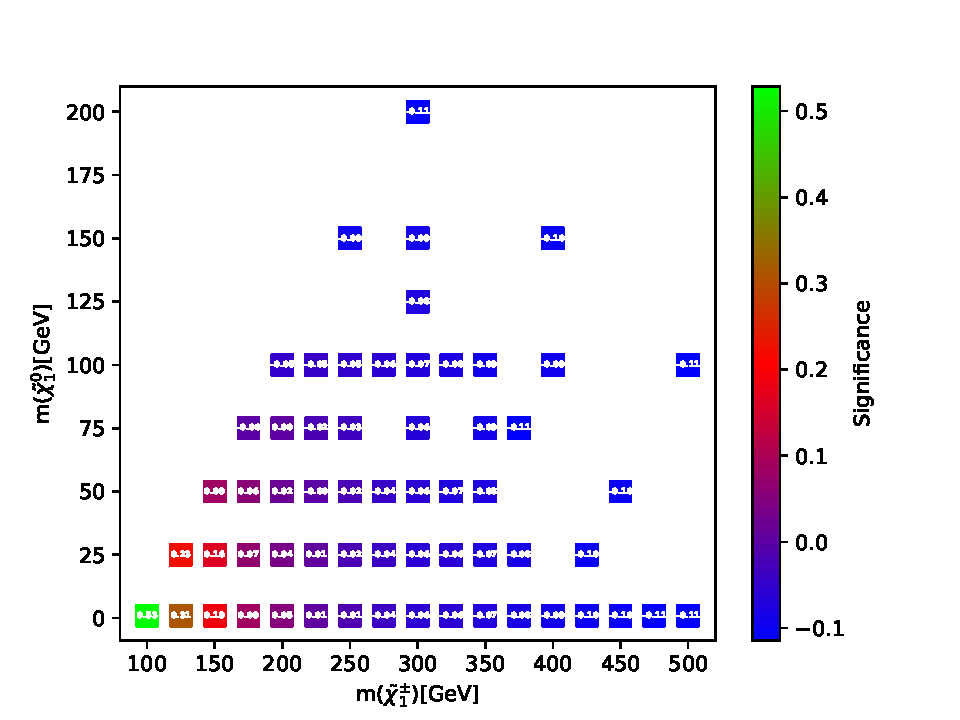
\includegraphics[width = \textwidth]{Figures/Significances/significance_BDT_WW_Low_level.pdf}
    \caption{Boosted Decision Tree.}
        \label{fig:signLowWWBDT}
    \end{subfigure}      
    \begin{subfigure}[t!]{0.49\textwidth}
    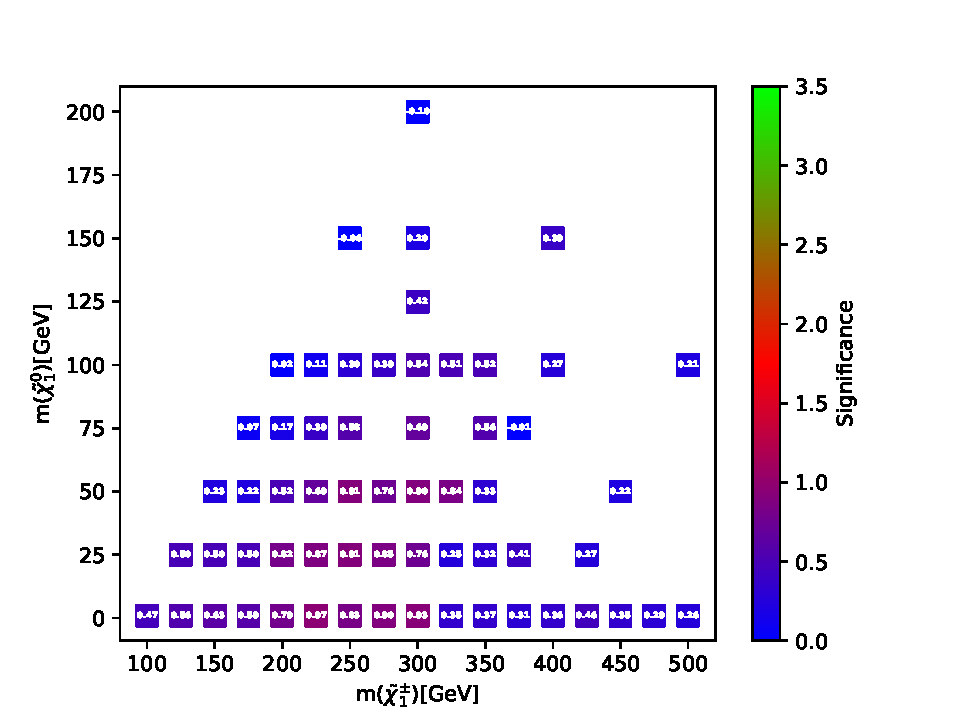
\includegraphics[width = \textwidth]{Figures/Significances/significance_NN_WW_Low_level.pdf}
    \caption{Neural Network.}
        \label{fig:signLowWWNN}
    \end{subfigure}
    \caption{Significance plots for chargino production with W-boson-mediated-decay where low level features are used during training the ML models.}
    \label{fig:signLowWW}
\end{figure}

\subsection{High level features}

\begin{figure}[H]
    \centering
    \begin{subfigure}[t!]{0.49\textwidth}
    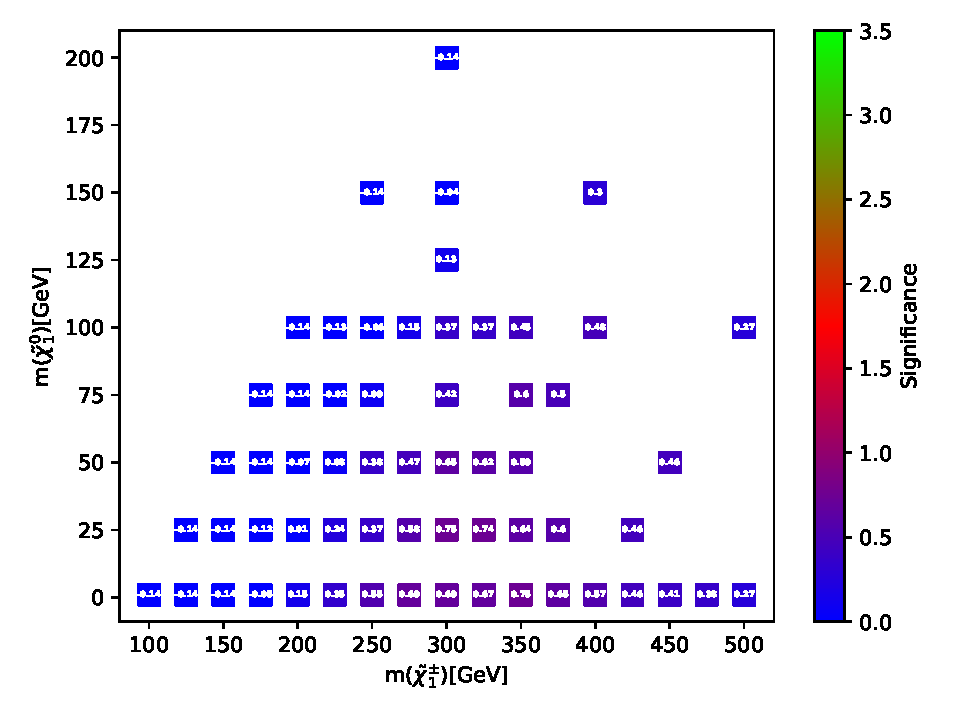
\includegraphics[width = \textwidth]{Figures/Significances/significanceCutandCount_WW_all.pdf}
    \caption{Cut and count.}
        \label{fig:signHighWWcandc}
    \end{subfigure}
    \\
    \begin{subfigure}[t!]{0.49\textwidth}
    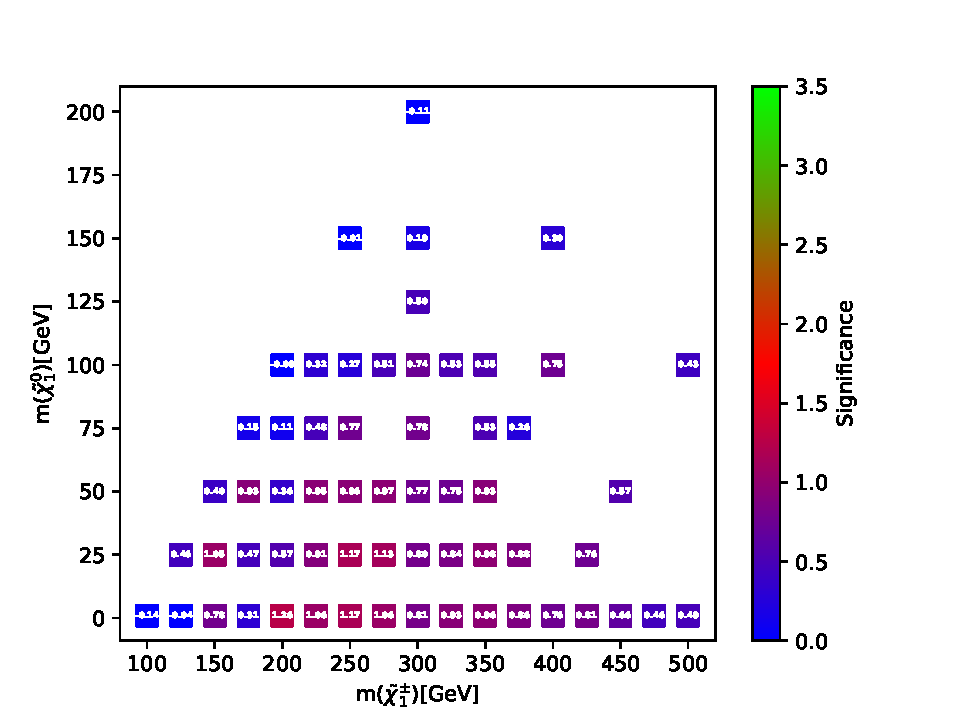
\includegraphics[width = \textwidth]{Figures/Significances/significance_BDT_WW_High_level.pdf}
    \caption{Boosted Decision Tree.}
        \label{fig:signHighWWBDT}
    \end{subfigure}      
    \begin{subfigure}[t!]{0.49\textwidth}
    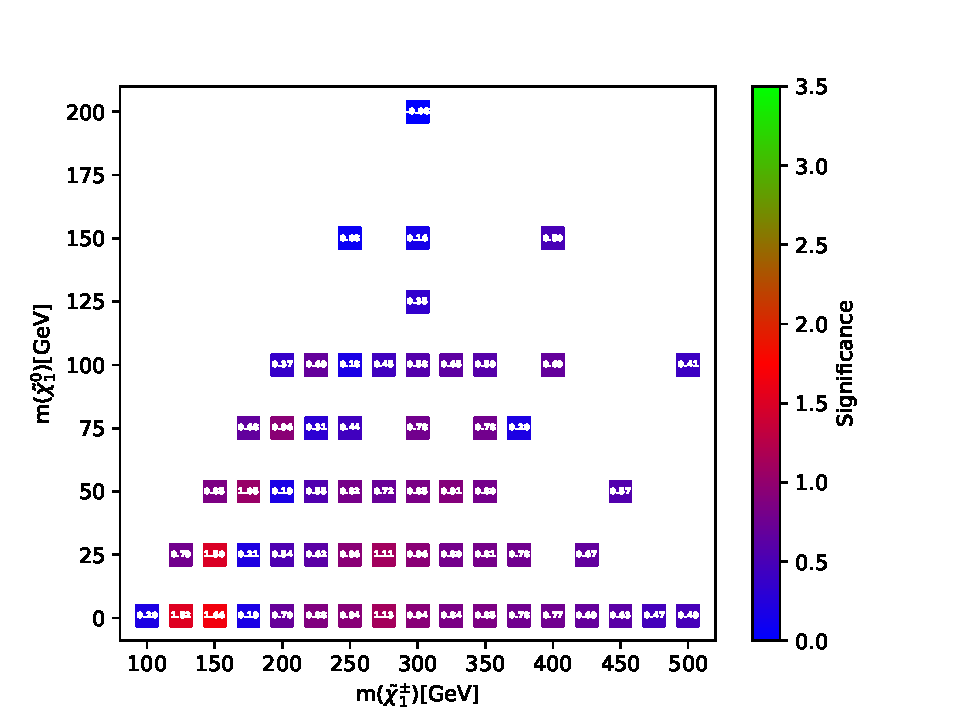
\includegraphics[width = \textwidth]{Figures/Significances/significance_NN_WW_High_level.pdf}
    \caption{Neural Network.}
        \label{fig:signHighWWNN}
    \end{subfigure}
    \caption{Significance plots for chargino production with W-boson-mediated-decay where high level features are used during training the ML models.}
    \label{fig:signHighWW}
\end{figure}








\section{Mono-Z}


\subsection{Low level features}

\begin{figure}[H]
    \centering
    \begin{subfigure}[t!]{0.49\textwidth}
    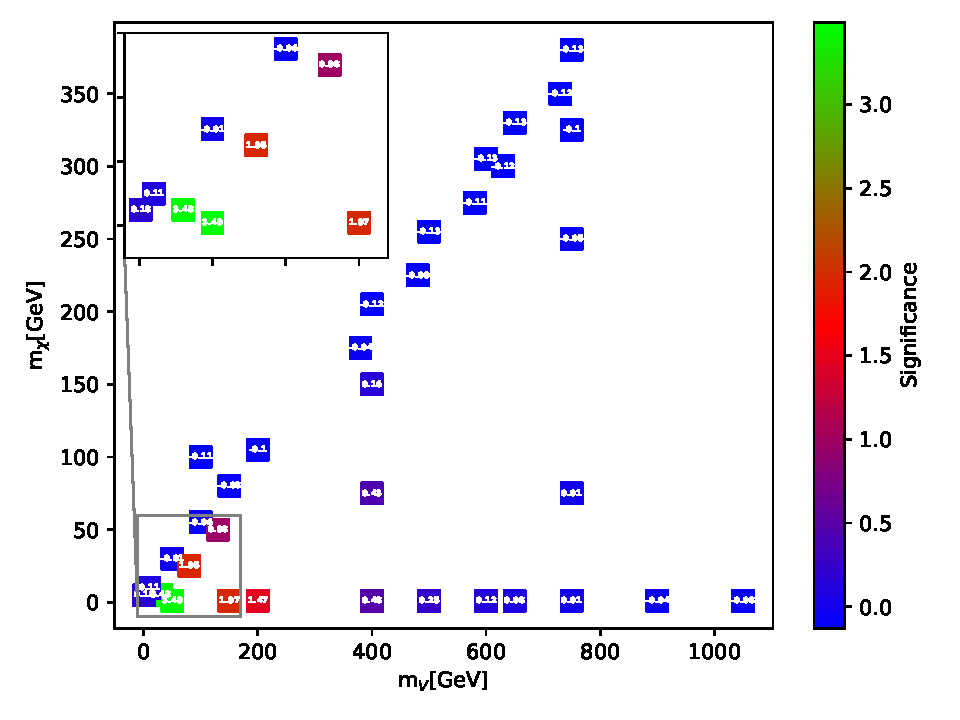
\includegraphics[width = \textwidth]{Figures/Significances/significanceCutandCount_monoZ_all.pdf}
    \caption{Cut and count.}
        \label{fig:signLowmonoZcandc}
    \end{subfigure}
    \\
    \begin{subfigure}[t!]{0.49\textwidth}
    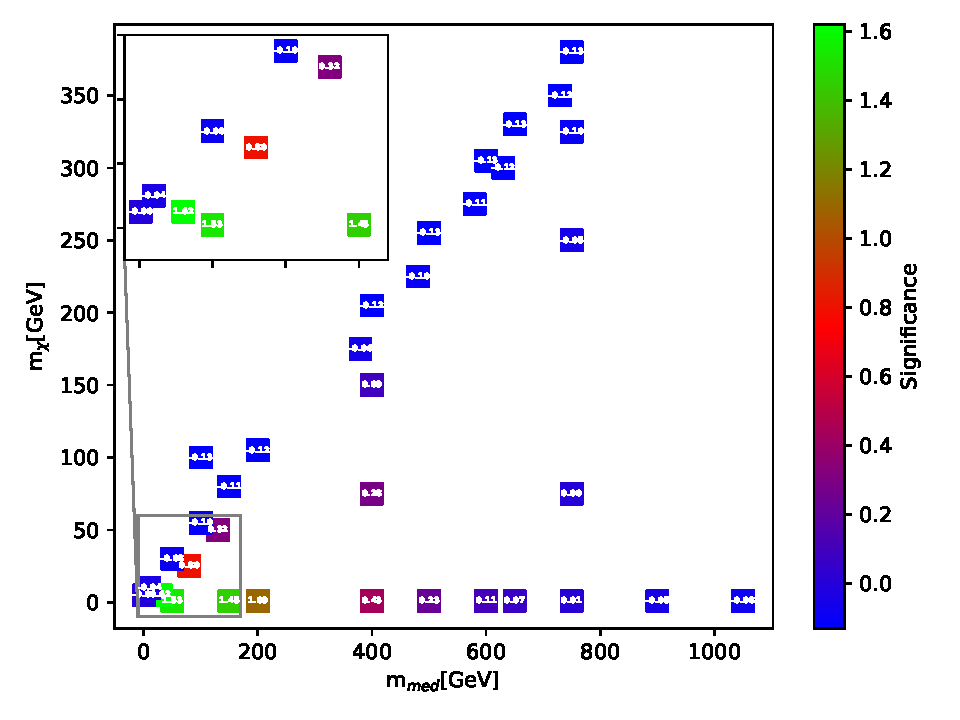
\includegraphics[width = \textwidth]{Figures/Significances/significance_BDT_monoZ_Low_level.pdf}
    \caption{Boosted Decision Tree.}
        \label{fig:signLowmonoZBDT}
    \end{subfigure}      
    \begin{subfigure}[t!]{0.49\textwidth}
    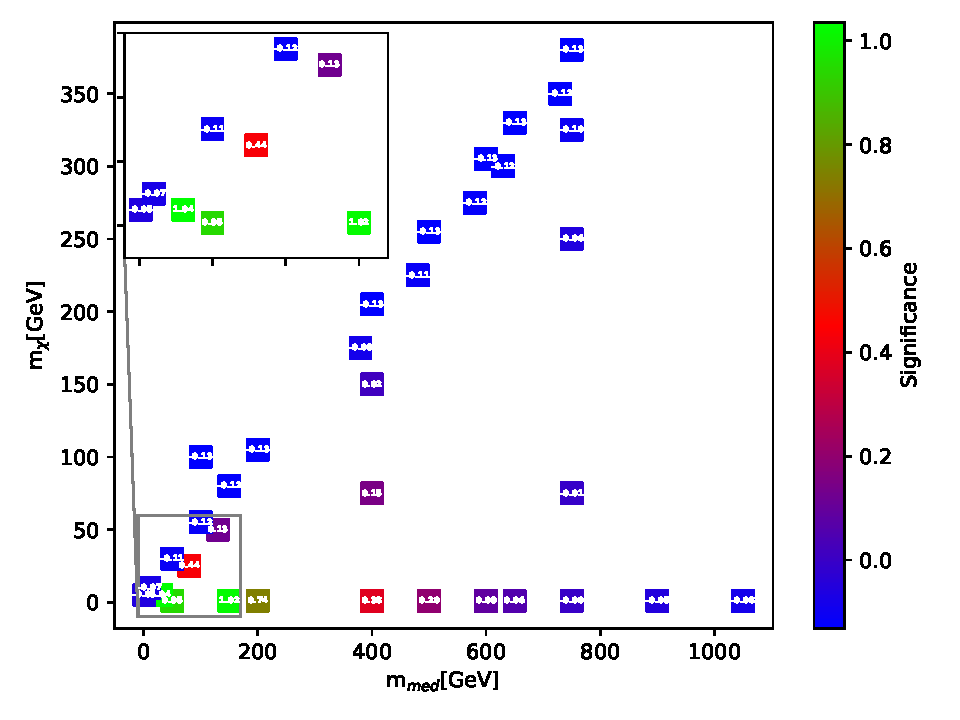
\includegraphics[width = \textwidth]{Figures/Significances/significance_NN_monoZ_Low_level.pdf}
    \caption{Neural Network.}
        \label{fig:signLowmonoZNN}
    \end{subfigure}
    \caption{Significance plots for the mono-Z process where low level features are used during training the ML models.}
    \label{fig:signLowmonoZ}
\end{figure}


\subsection{High level features}

\begin{figure}[H]
    \centering
    \begin{subfigure}[t!]{0.49\textwidth}
    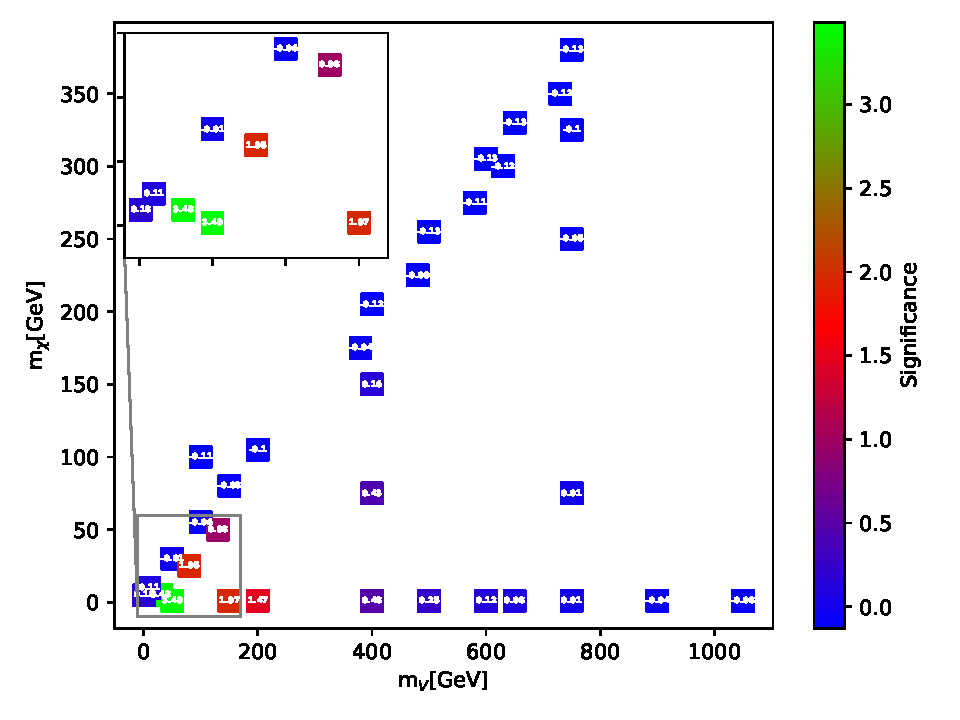
\includegraphics[width = \textwidth]{Figures/Significances/significanceCutandCount_monoZ_all.pdf}
    \caption{Cut and count.}
        \label{fig:signHighmonoZcandc}
    \end{subfigure}
    \\
    \begin{subfigure}[t!]{0.49\textwidth}
    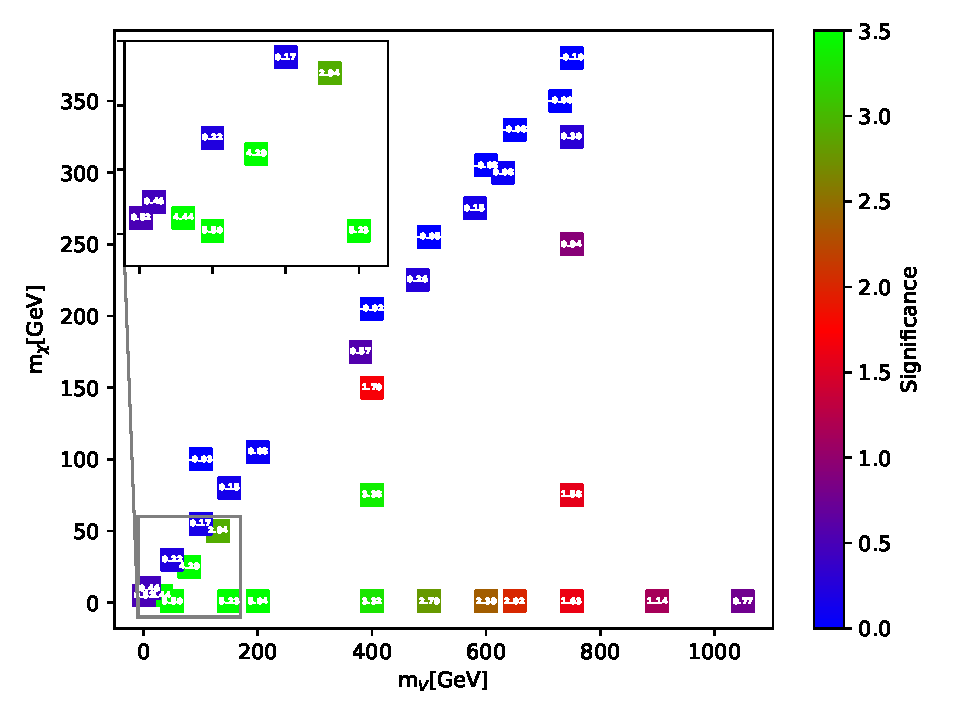
\includegraphics[width = \textwidth]{Figures/Significances/significance_BDT_monoZ_High_level.pdf}
    \caption{Boosted Decision Tree.}
        \label{fig:signHighmonoZBDT}
    \end{subfigure}      
    \begin{subfigure}[t!]{0.49\textwidth}
    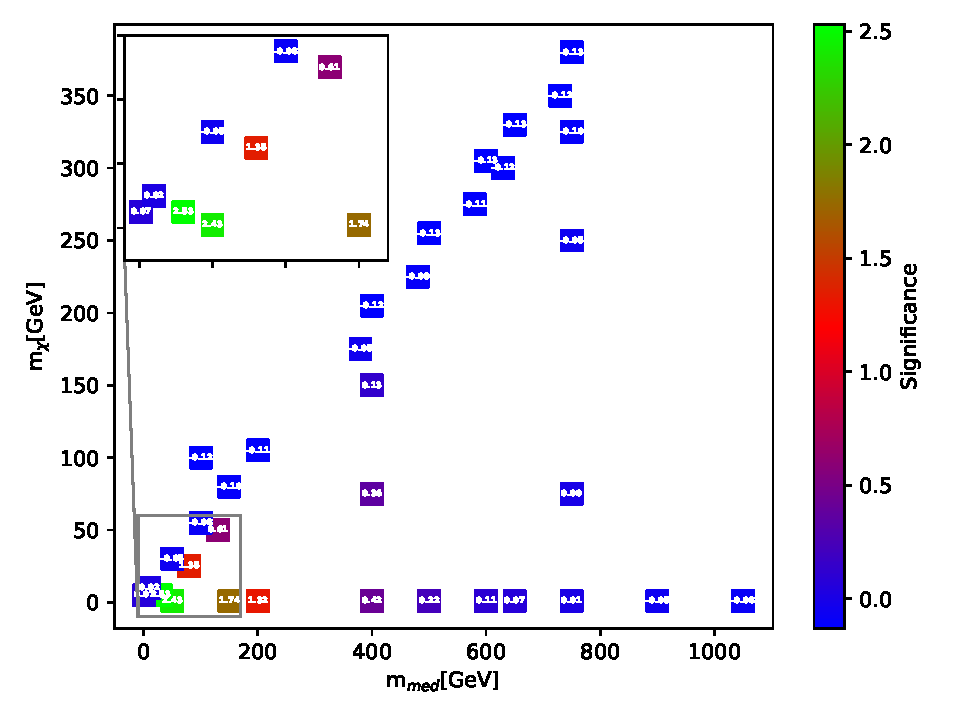
\includegraphics[width = \textwidth]{Figures/Significances/significance_NN_monoZ_High_level.pdf}
    \caption{Neural Network.}
        \label{fig:signHighmonoZNN}
    \end{subfigure}
    \caption{Significance plots for the mono-Z process where high level features are used during training the ML models.}
    \label{fig:signHighmonoZ}
\end{figure}


